\documentclass[11pt]{article}
\usepackage[sort]{natbib}
\usepackage{bm,amsmath,bbm,amsfonts,nicefrac,latexsym,amsmath,amsfonts,amsbsy,amscd,amsxtra,amsgen,amsopn,bbm,amsthm,amssymb,graphicx}
\usepackage{fancyhdr}
\usepackage[margin=1.0in]{geometry}
\usepackage[section]{placeins}
\bibliographystyle{abbrvnat}

\title{Thesis Introduction}
\author{Ewan Pinnington}

\newtheorem{theorem}{Theorem}[section]
\newtheorem*{defn}{Definition}


\begin{document}

\maketitle

\section{Notation}
List of symbols and meanings consistent throughout thesis.

\section{The global carbon cycle}

\begin{figure}[ht]
    \centering
    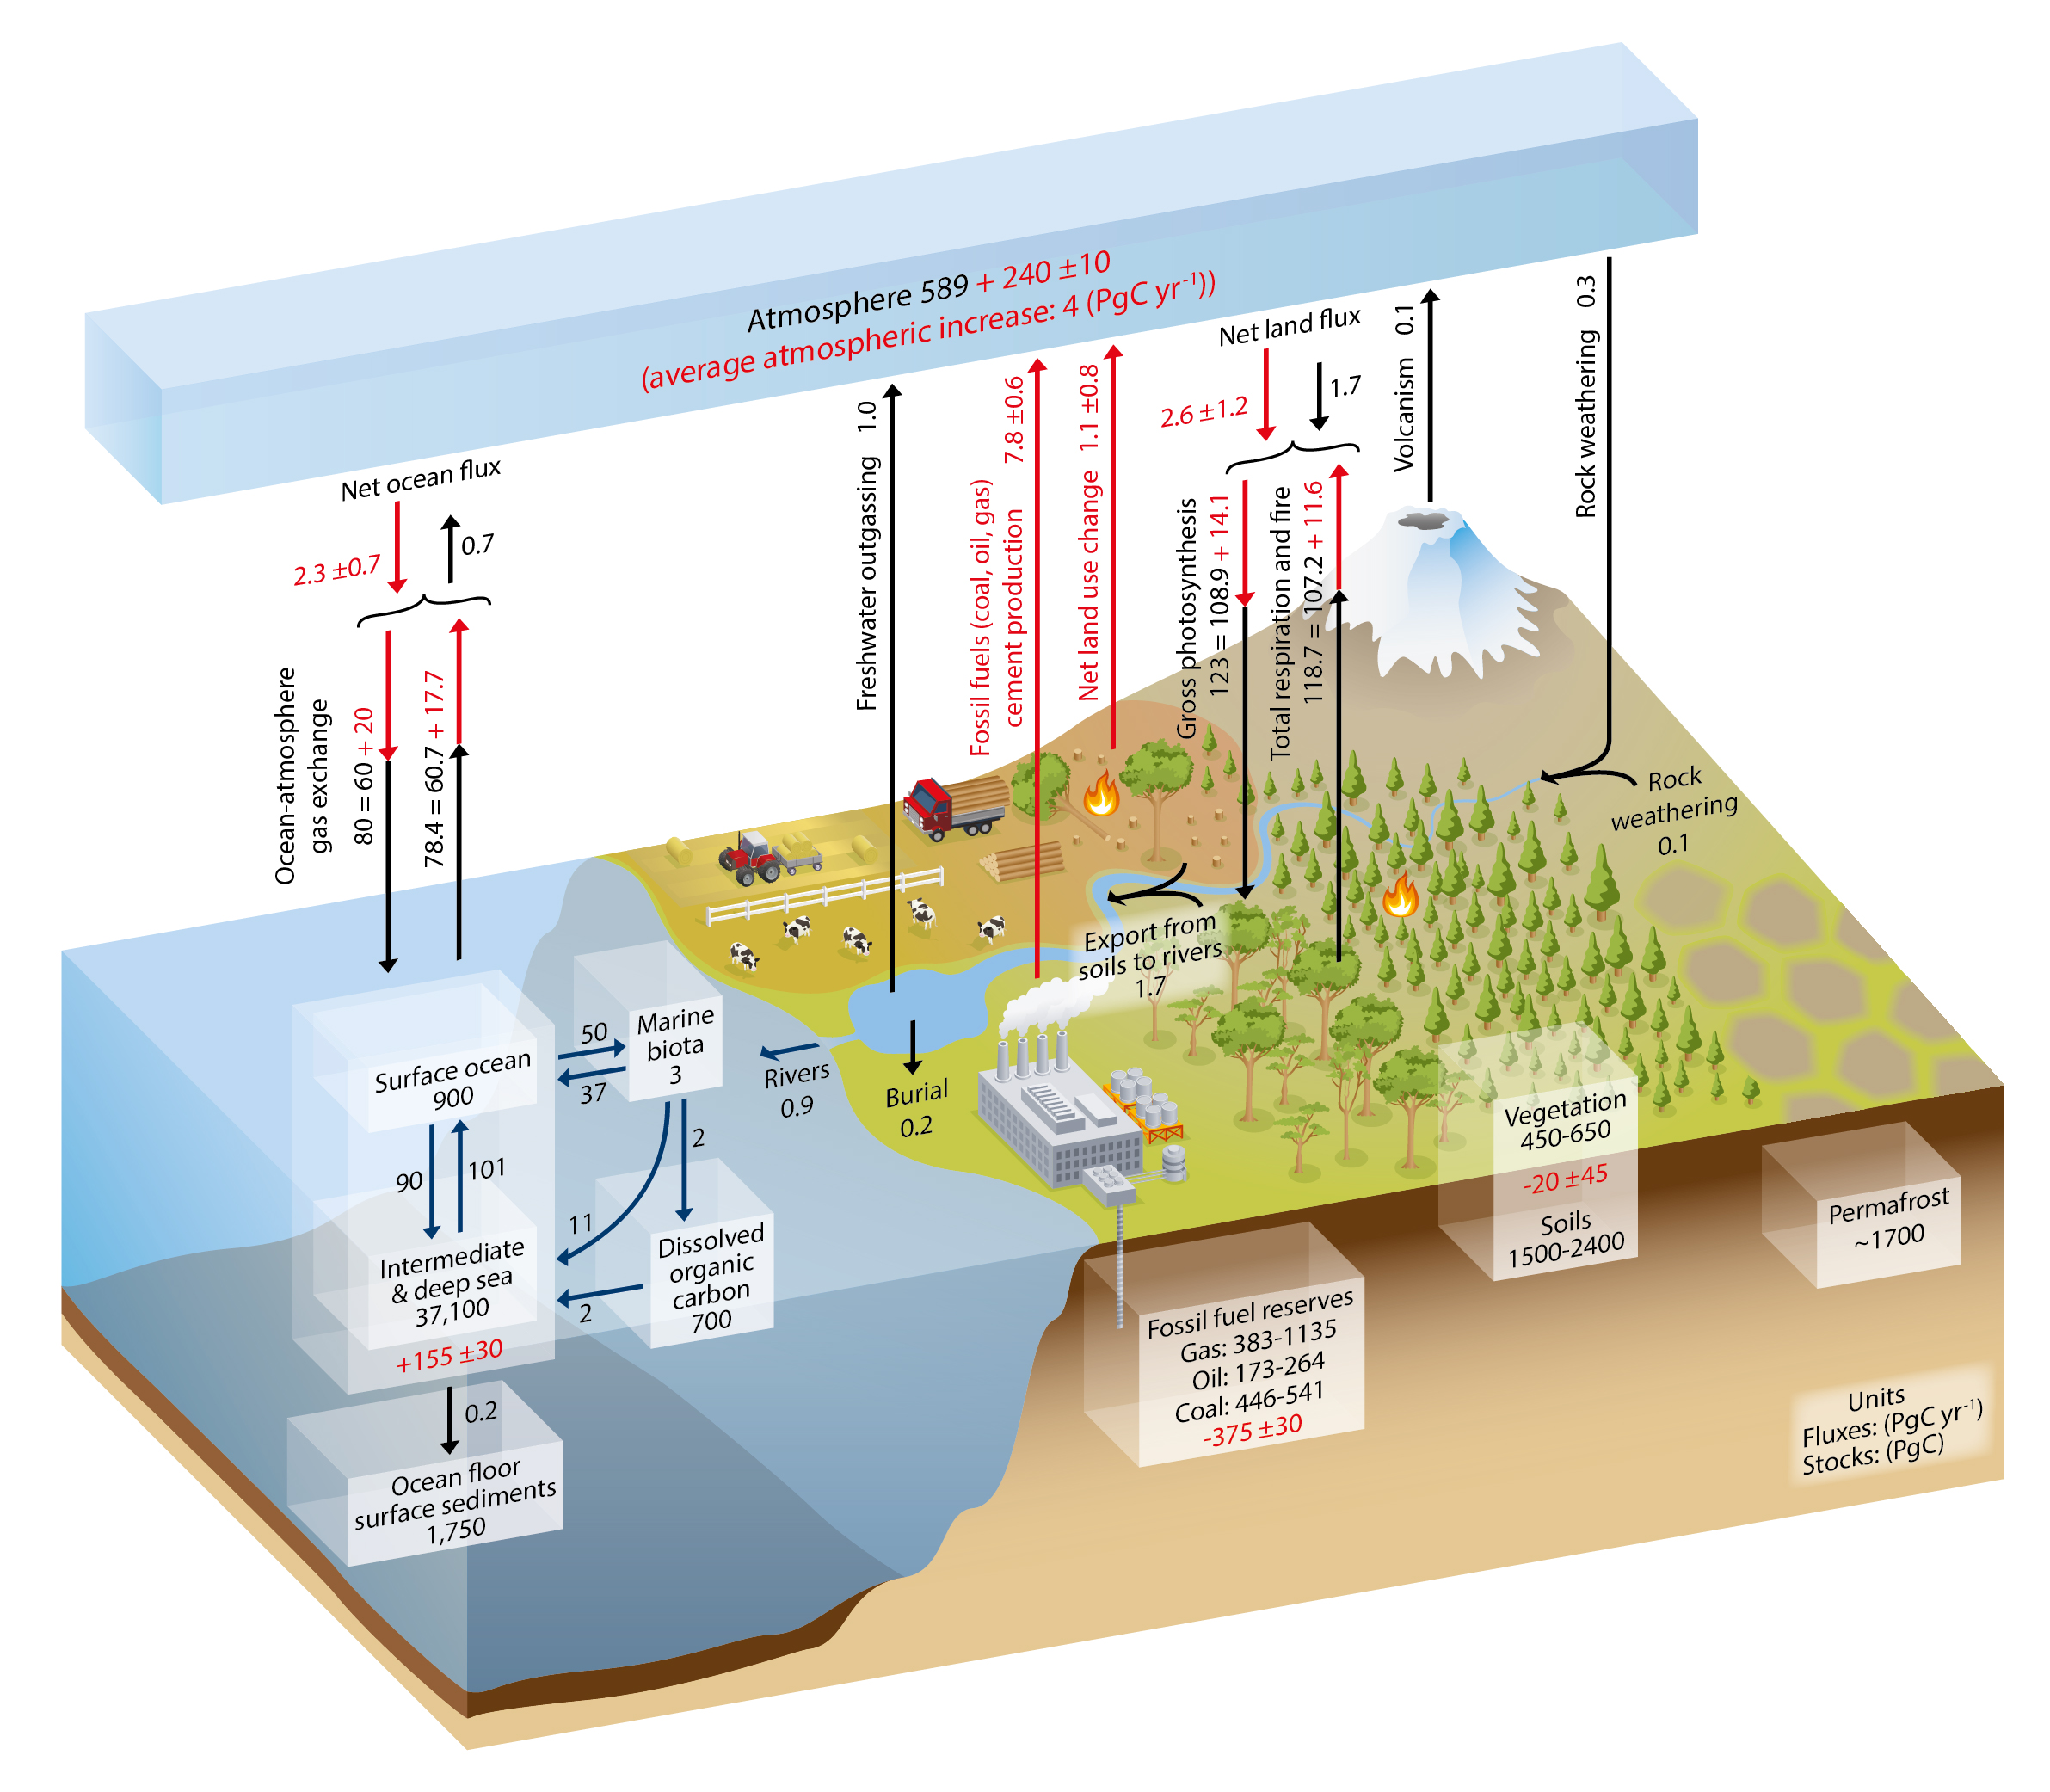
\includegraphics[width=0.9\textwidth]{ipcc_fig6_1.jpg}
    \caption{Global carbon cycle simplified schematic \citep{ciais2014carbon}. Black numbers and arrows represent reservoir mass and exchange fluxes estimated for the time prior to the industrial era (~1750). Red numbers and arrows represent annual fluxes average over the 2000-2009 time period. Red numbers in the rservoirs indicate the cumulative change of carbon over the industrial period (1750-2011).}
    \label{fig:ipcc_fig6.1}
\end{figure}

IPCC figure 6.1 and 6.8: Partitioning of fluxes important and hard (shown by error on estimates in fig 6.1). Land surface carbon uptake least understood mechanism in the global carbon cycle, ref IPCC. Will uptake remain the same under climate change.

\section{The role of models}

\begin{figure}[ht]
    \centering
    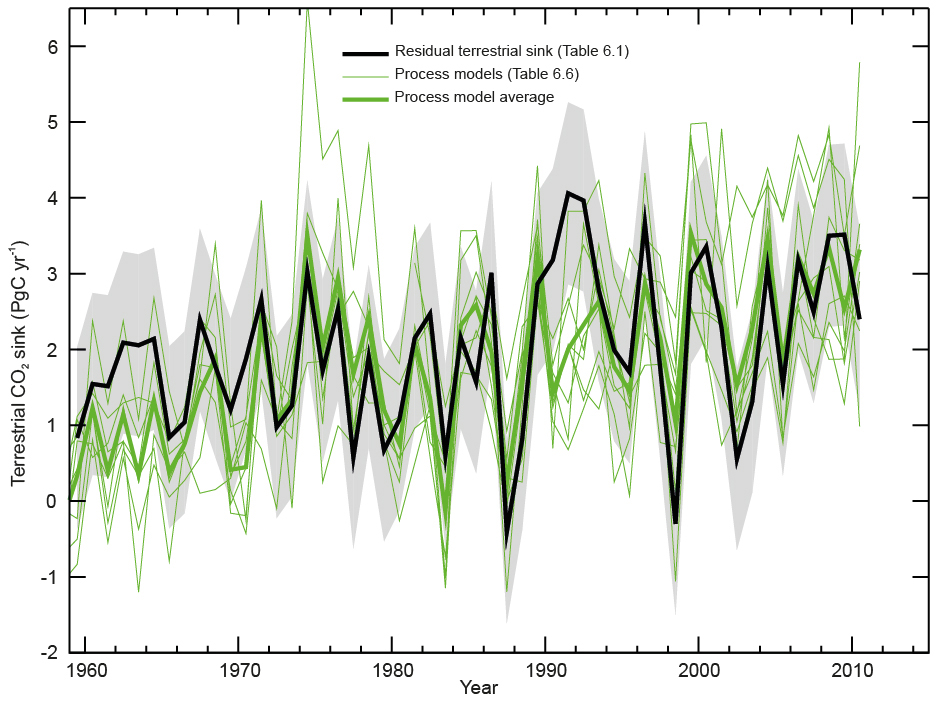
\includegraphics[width=0.9\textwidth]{ipcc_fig6_16.jpg}
    \caption{Modelled land sink \citep{ciais2014carbon}.}
    \label{fig:ipcc_fig6.1}
\end{figure}

IPCC figure 6.16 and section 6.3.2.6.6: Contribution of models to understanding the terrestrial carbon cycle. Reference every DALEC paper.

\section{Eddy covariance and other observations}

Baldocchi paper: Many observations of forest carbon flux made worldwide.

\section{Data assimilation}

Role of DA in NWP improving forecast skill. 


\bibliography{../PhD}{}
\end{document}